\documentclass{TEMA}
\usepackage[utf8]{inputenc}
\usepackage[brazil]{babel}      % para texto em Português
\usepackage{amsfonts}
\usepackage{amsmath,amssymb}
\usepackage{graphicx}
\usepackage{xcolor}
\usepackage[ruled]{algorithm2e}
\usepackage{algorithmic}
%\usepackage{algpseudocode}
\usepackage{hyperref}
\newcommand{\Z}{\mathbb{Z}}

\title{Atividade 3 - Grupo 8 - MO824}

\author{
    André Soranzzo Mota          - RA 166404\\
    Victor Ferreira Ferrari      - RA 187890\\
    Gabriel Oliveira dos Santos  - RA 197460
}

\begin{document}

\criartitulo

\runningheads{A.S. Mota, V.F. Ferrari e G.O. dos Santos}%
{Atividade 3}

\begin{abstract}
{\bf Resumo}. Este documento apresenta uma relaxação lagrangiana para o 2-TSP, que visa encontrar dois ciclos hamiltonianos com conjuntos distintos de arestas e cuja soma de peso dessas arestas seja mínima. O modelo matemático é apresentado, assim como o processo de obtenção do custo lagrangiano, o método de subgradientes utilizado para obtenção de limitantes duais, e a heurística lagrangiana criada para transformar o dual em uma solução viável para o 2-TSP. Foi realizado a geração de instâncias através de um \textit{script} em \emph{Python} e do software Gurobi. A relaxação lagrangiana forneceu melhores limitantes, porém estourou mais facilmente o tempo limite de execução, possivelmente devido ao tempo exponencial da heurística. O modelo linear inteiro retornou o resultado ótimo, mas aumentou muito tempo de execução conforme aumentamos o tamanho da instância.

{\bf Palavras-chave}. Relaxação Lagrangiana, Otimização, 2-TSP, Heurística.

\end{abstract}

\section{Introdução}

    Este trabalho consiste na apresentação de uma relaxação lagrangiana para o problema proposto na Atividade 3 de MO824 2S-2020, e da realização de testes em comparação com a resolução direta do modelo matemático original para o problema.
    
    Chamado 2-TSP, o problema é uma variação do tradicional TSP (\textit{travelling salesman problem}) e busca encontrar dois ciclos hamiltonianos com conjuntos de arestas disjuntos e cuja soma de peso dessas arestas seja mínima.
    
    Para testar o modelo relaxado, foi utilizado o método de subgradientes, baseado no material apresentado em aula e pelo artigo de John E. Beasley \cite{beasley}. As técnicas retiradas do artigo serão devidamente apontadas.

\section{Modelo Matemático}
    A seguinte variável foi usada no modelo:
    
    $x_{e}^k$: Variável de decisão binária associada à presença ($x_e = 1$) ou não ($x_e = 0$) da aresta $e$ no ciclo $k$, para $k \in \{1,2\}$ e $e \in E$.\\
    
    O modelo original do 2-TSP pode ser visto a seguir.
    \begin{equation*}
    \begin{array}{ll@{}ll@{}ll}
    \text{min}  & \displaystyle\sum\limits_{k \in \{1,2\}}\sum\limits_{e \in E} c_{e}x_{e}^k  & &(1)\\
    \text{s.a}       & \displaystyle\sum\limits_{e \in \delta(i)} x_{e}^k = 2 & \forall i \in V,                        \forall k \in \{1,2\} &(2)\\
                     & \displaystyle\sum\limits_{e \in E(S)} x_{e}^k \leq |S|-1 & \forall S \subset V, \forall k \in \{1,2\} &(3)\\
                     & \displaystyle\sum\limits_{k \in \{1,2\}} x_{e}^k \leq 1 & \forall e \in E &(4)\\
                     & x_{e}^k \in \{0,1\} & \forall e \in E, \forall k \in \{1,2\} &(5)\\
    \end{array}
    \end{equation*}
    
    Onde $\delta(i)$ é o conjunto de arestas incidentes no vértice $i$, $S \subset V$ é um subconjunto próprio de vértices e $E(S)$ é o conjunto das arestas cujas extremidades estão em $S$.\\
    
    Dualizando o conjunto de restrições $(4)$ e introduzindo os multiplicadores de Lagrange para cada restrição ($\forall e \in E$), temos uma relaxação para o 2-TSP, com função objetivo:
    \begin{equation*}
        \text{min} \displaystyle\sum\limits_{k \in \{1,2\}}\sum\limits_{e \in E} c_{e}x_{e}^k  + \sum\limits_{e \in E} \lambda_{e} (\sum\limits_{k \in \{1,2\}} x_{e}^k - 1)
    \end{equation*}
    
    que podemos simplificar para:
    
    \begin{equation*}
        \text{min} \displaystyle\sum\limits_{k \in \{1,2\}}\sum\limits_{e \in E} (c_{e}+\lambda_e)x_{e}^k - \sum\limits_{e \in E} \lambda_e
    \end{equation*}
    
    Assim, o LLBP para o 2-TSP é o seguinte:
    
    \begin{equation*}
    \begin{array}{ll@{}ll@{}ll}
    \text{min}  & \displaystyle\sum\limits_{k \in \{1,2\}}\sum\limits_{e \in E} C_{e}x_{e}^k - \sum\limits_{e \in E} \lambda_e & &(1)\\
    \text{s.a}       & \displaystyle\sum\limits_{e \in \delta(i)} x_{e}^k = 2 & \forall i \in V,                        \forall k \in \{1,2\} &(2)\\
                     & \displaystyle\sum\limits_{e \in E(S)} x_{e}^k \leq |S|-1 & \forall S \subset V, \forall k \in \{1,2\} &(3)\\
                     & x_{e}^k \in \{0,1\} & \forall e \in E, \forall k \in \{1,2\} &(5)\\
    \end{array}
    \end{equation*}
    
    onde $C_e$ é o custo lagrangiano do problema, dado por $c_e + \lambda_e~\forall e \in E$.
    
    O método de subgradientes consiste em otimizar os multiplicadores de Lagrange para encontrar o melhor limitante dual (ou seja, resolver o problema dual lagrangiano) ao deslocar na direção do subgradiente da função objetivo em relação a $\lambda$. Uma componente do subgradiente é:
    \begin{equation*}
        \tag{GRAD}
        g_e = \displaystyle\sum\limits_{k \in \{1,2\}} (x_{e}^k - 1)
        \label{eqn::grad}
    \end{equation*}

\section{Implementação} \label{imp}

A implementação da solução foi feita em \emph{Python}, por meio da construção de um "framework". Uma função genérica que realiza a execução do método de subgradientes recebe um objeto de tipo "Problem", classe abstrata que fornece uma série de métodos que devem ser implementados em classes filhas. O método segue o pseudocódigo visto em aula, com adições propostas em \cite{beasley}.

\subsection{Método de Subgradientes}
A função objetivo do LLBP consiste da subtração entre dois termos. Como um desses termos é linear, não dependendo das variáveis do problema, não tem impacto na resolução do problema. Assim, ele pode ser adicionado apenas no resultado final. Uma descrição em alto nível do método utilizado pode ser visto no Algoritmo \ref{alg::subgradient}.

\begin{algorithm}[H]
    \label{alg::subgradient}
    \caption{Método de Subgradientes}
    \begin{algorithmic}[1]
        \STATE Inicialize valores de controle ($\pi, t_0$) e multiplicadores $\lambda_e~\forall e \in E$.
        \STATE Calcule os custos lagrangianos com o conjunto atual de multiplicadores $\lambda^{(k)}$.
        \STATE Resolva o 2-TSP sem a restrição que garante que os ciclos sejam aresta-disjuntos, obtendo uma solução $x^{(k)}$.
        \STATE Subtraia a soma dos multiplicadores do conjunto atual do custo da solução, para obter o limitante dual $Z_{L}^{(k)}$ para o 2-TSP.
        \STATE Utilize a heurística lagrangiana vista em Algorithm \ref{alg::heuristic} para obter um limitante primal $Z_{U}^{(k)}$.
        \STATE Calcule o conjunto de subgradientes $g_e^{(k)}$ segundo a equação \eqref{eqn::grad}, a partir de $x^{(k)}$.
        \STATE Calcule o passo, dado por $\alpha^{(k)} = \pi\frac{(1+\varepsilon)Z_{U}^{(k)} - Z_{L}^{(k)}}{(\sum_{e \in E} g_e^{(k)})^2}$
        \STATE Atualize o conjunto de multiplicadores: $\lambda_e^{(k+1)} = \text{max}(0, \lambda_e^{(k)} + \alpha^{(k)}g_e^{(k)})$.
        \STATE Retorne ao passo 2 até que um dos critérios de parada seja atendido.
        \STATE Devolva os melhores limitantes dual e primal, com a melhor solução encontrada.
    \end{algorithmic}
\end{algorithm}

Entre os passos 4 e 5, o valor de $\pi$ é reduzido pela metade a cada $m$ iterações, iniciando com um valor $\pi_0$. Esses valores foram fixados em $\pi_0=2, m=30$ \cite{beasley}. No passo 7, um fator $1+\varepsilon$ multiplica o limitante primal para evitar que $\alpha$ fique muito pequeno \cite{beasley}. $\varepsilon$ é fixado em 0.0005. Os multiplicadores são inicializados com zero, valor escolhido arbitrariamente.

Os critérios de parada utilizados incluem tempo limite, otimalidade da solução encontrada, valor mínimo de $\pi$ (limite de iterações), e \textbf{convergência}. Esse último critério ocorre quando todos os componentes do subgradiente são iguais a zero, ou seja, os multiplicadores não sofrerão alteração. Nesse caso, se a solução dual for viável para o problema original, é a solução ótima do problema \cite{beasley}. Ligado a isso, se em uma determinada iteração um multiplicador $\lambda_e^{(k)}$ tem valor zero e a componente correspondente do subgradiente for negativa, pelo passo 8 o multiplicador não sofrerá alteração. Por isso, pode-se igualar aquela componente a zero \cite{beasley}.

\subsection{Heurística Lagrangiana}

Implementamos nossa heurística baseada na modelagem do TSP no Gurobi. Dados dois ciclos hamiltonianos $c_1$ e $c_2$, escolhemos o ciclo de menor custo, e desconsideramos o outro. Após isso, removemos do grafo as arestas que fazem parte do ciclo que foi mantido, e executamos o algoritmo que resolve o TSP usando o Gurobi para o grafo resultante. Dessa forma, ao término da execução do algoritmo temos dois ciclos hamiltonianos com conjuntos disjuntos de arestas, sendo, portanto, uma solução viável para o 2-TSP. Abaixo é apresentado o pseudo-código, Algoritmo \ref{alg::heuristic}.

\begin{algorithm}[H]
    \label{alg::heuristic}
    \caption{Heurística Lagrangiana}
    \begin{algorithmic}[1]
        \REQUIRE grafo não direcionado G = (V, E) e ciclos hamiltonianos $c_1$ e $c_2$
        \STATE ciclo $\leftarrow \emptyset$
        \IF{custo($c_1$) < custo($c_2$)}
            \STATE ciclo $\leftarrow c_1$
        \ELSE
            \STATE ciclo $\leftarrow c_2$
        \ENDIF
        
        \FORALL{$(u, v) \in$ ciclo}
            \STATE remova $(u, v)$ de E
        \ENDFOR
        \STATE $ciclo_{novo} \leftarrow$ TSP(G)
        
        \RETURN ciclo, $ciclo_{novo}$
        
    \end{algorithmic}
\end{algorithm}

%\subsection{Avaliação}

%  \begin{figure}[htp!]
%     \centering
%     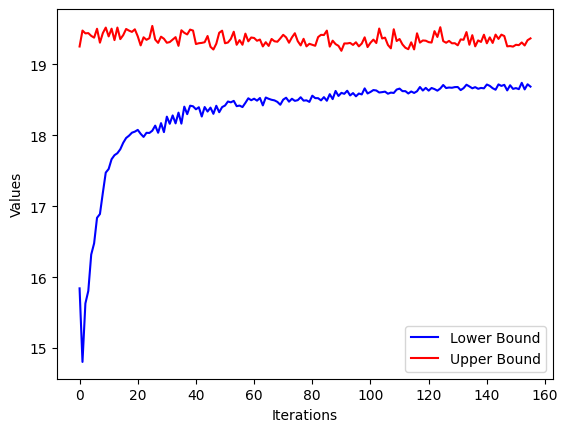
\includegraphics[scale=0.45]{bounds_graph.png}
%     \caption{Limitantes inferior e superior ao longo das iterações do algoritmo considerando uma instância de 100 nós.}
%     \label{fig:bounds_graph}
% \end{figure}  


\section{Metodologia de Avaliação}
\subsection{Gerador de Instâncias}
        As instâncias foram geradas de maneira aleatória e uniforme a partir de uma quantidade de cidades fornecida e uma \textit{random seed}. Como proposto, as cidades foram posicionadas aleatoriamente no plano, e as distâncias euclideanas entre os pares foram calculadas. A geração é feita no arquivo \texttt{generator.py}, e todas as instâncias foram executadas com a mesma \textit{seed}.
\subsection{Especificações do Computador}
    As especificações de hardware do computador no qual foram feitas as execuções estão na \tablename~\ref{table:conditions}.
    
    % \begin{figure}[htp!]
    % \caption{}
    % \centering
    % 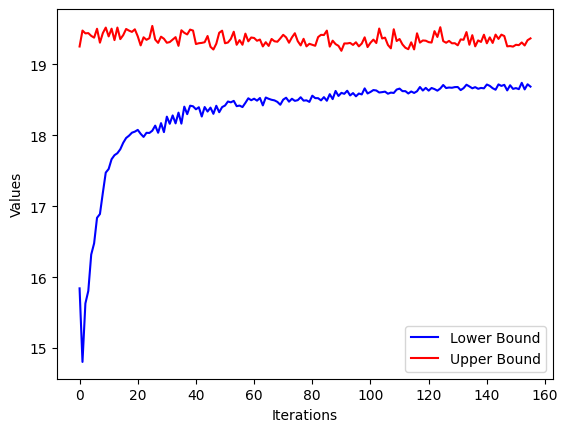
\includegraphics[width=0.6\textwidth]{bounds_graph.png}
    % \end{figure}
    \vspace{-0.3cm}
    \begin{table}[ht!]
        \centering
        \caption{Condições de Execução}
        \label{table:conditions}
        \vspace{0.3cm}
        \resizebox{70ex}{!}{
        \begin{tabular}{|c|c|}
        \hline
            Modelo da CPU & AMD Ryzen 5 2500U (4C/8T)\\ \hline
            Frequência do Clock da CPU & 2.00 GHz\\ \hline
            RAM & 12 GB/2400 MHz \\ 
        \hline
        \end{tabular}
        }
    \end{table}
    
    O sistema operacional utilizado foi o Ubuntu 20.04.1 LTS. Foi utilizado como software de execução o \textit{solver} Gurobi Optimizer V9.0.3. Os modelos foram executados com limite de 1800 segundos (30 minutos) e sem limite de memória.
\vspace{-0.18cm}
\section{Resultados Obtidos e Análise}
        Para cada tamanho proposto na atividade foi gerada uma instância e os resultados alcançados estão na \tablename~\ref{table:resultados}. 
        \vspace{-0.5cm}
        
        \begin{table}[ht]
                \caption{Resultados Obtidos}
                \label{table:resultados}
                \vspace{0.3cm}
                \centering
                \resizebox{\textwidth}{!}{%
                \begin{tabular}{|c|c|c|c|c|c|c|}
                \hline
                Instância &
                  \begin{tabular}[c]{@{}c@{}}PLI \\ Limite Inferior\end{tabular} &
                  \begin{tabular}[c]{@{}c@{}}PLI \\ Limite Superior\end{tabular} &
                  \begin{tabular}[c]{@{}c@{}}PLI \\ Tempo de Execução (s)\end{tabular} &
                  \begin{tabular}[c]{@{}c@{}}Relaxação Lagrangiana\\ Limite Inferior\end{tabular} &
                  \begin{tabular}[c]{@{}c@{}}Relaxação Lagrangiana\\ Limite Superior\end{tabular} &
                  \begin{tabular}[c]{@{}c@{}}Relaxação Lagrangiana\\ Tempo de Execução (s)\end{tabular} \\ \hline
                100 & 19,1645 & 19,1660 & 112,9264  & 18,2633 & 19,3054 & 205,8787  \\ \hline
                150 & 22,8620 & 22,8620 & 471,1312  & 21,7847 & 23,0409 & 1800,2839 \\ \hline
                200 & 25,9125 & 25,9143 & 1404,9435 & 23,1658 & 26,2486 & 1800,6086 \\ \hline
                250 & 28,4179 & 36,7105 & 1800,0144 & 24,4823 & 29,0124 & 1802,1623 \\ \hline
                300 & 31,6393 & inf     & 1800,1609 & 26,1999 & 32,2801 & 1800,9896 \\ \hline
                \end{tabular}%
                }
        \end{table}
    
        A partir da \tablename~\ref{table:resultados} podemos observar que para instâncias menores dos problema  (200 vértices ou menos) o algoritmo de Programação Linear Inteira (PLI) encontra facilmente a solução ótima em menos de 30 minutos. Entretanto, para instâncias maiores o algoritmo estoura o tempo limite de execução, de 30 minutos, e tem uma parada forçada retornando limitantes inferior e superior não tão bons. Nesse cenário o método de relaxação lagrangiana se apresenta uma abordagem melhor, note que mesmo estourando o tempo limite, são retornados limitantes melhores que o do modelo de PLI. Especificamente para a instância com 300 vértices, o modelo de PLI sequer conseguiu encontrar algum limitante superior, enquanto a relaxação lagrangiana retornou os limitantes 26.1999 e 32.2801.
        
        De modo geral, pode-se dizer que a abordagem usando o método de subgradientes estoura mais facilmente o tempo limite, mas isso se deve ao fato de nossa heurística também ter tempo exponencial. Assim, seria interessante tentar encontrar alguma heurística em tempo polinomial para tentar melhorar esse tempo de execução. Todavia, ainda com essa heurística que executa em tempo exponencial, conseguimos ter bons resultados para instâncias grandes (250 vértices ou mais).
        
        Observando os valores dos limitantes duais e primais encontrados ao longo do tempo, é perceptível a convergência ao ótimo, embora o método não tenha encontrado esse valor em nenhuma instância. 
        Nos testes feitos, apenas um conjunto de hiperparâmetros, descritos na seção \ref{imp}, foram usados. Modificando esses parâmetros, como o valor inicial dos multiplicadores, o valor de $\varepsilon$ ou o número de iterações até a divisão de $\pi$, é possível que resultados melhores sejam encontrados dentro do tempo limite.

\bibliographystyle{ieeetr}
\bibliography{ref}

\end{document}